\section{Method}

In this technical note we focus on developing an algorithm for reliably computing the optimal
leaf trajectories, given a candidate dose-rate trajectory.
We use linear splines for the dose-rate and leaf trajectories,
and avoid many of the issues with local minima by using a smooth model of how the leaves block radiation.

The inner optimization (leaf trajectories) is transcribed to a smooth non-linear program (NLP),
which can easily be solved using standard NLP solvers such as
FMINCON \cite{MatlabOptimizationToolbox2014}, SNOPT \cite{Snopt7}, or IPOPT \cite{Wachter2006}.

The outer optimization is still a difficult optimization, which is made somewhat non-smooth by
having an iterative optimization procedure inside the objective function.
As a result, it is likely that smooth solvers such as those used for the inner optimization would
have difficulty converging due to bad gradient estimates.
For the purposes of this technical note we decided to use CMAES \cite{Hansen2001},
a good general-purpose solver for difficult non-linear optimization problems.

\subsection{Trajectory Representation}

The final goal of our optimization is to compute three trajectories:
radiation dose-rate $r(t)$, lower leaf position $z_L(t)$, and upper leaf position $z_U(t)$.

As discussed in Section \S \ref{sec:WhyUseLinearSplines}, each of these trajectories is
represented by a piecewise linear spline. Each of the three trajectories shares the same set of
knot times $t_k \in \{t_0, t_1, \dots, t_N\}$, where $N$ is the number of knot points.
The value of the dose rate and leaf positions at knot time $t_k$ are given by
$r_k$, $x_{L,k}$, and $y_{U,k}$ respectively.
We assume that the total duration of the trajectory is given, although this could easily be made
a decision variable in the outer optimization when computing dose rate.

\begin{figure}
  \centering
  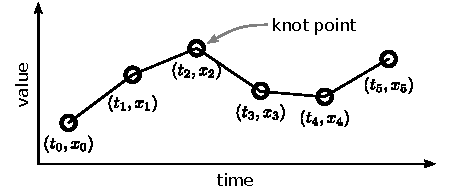
\includegraphics{fig/linearSpline.pdf}
  \caption{Linear Spline. We represent the dose-rate and leaf position trajectories as linear
           splines. A linear spline is fully defined by its value at the knot points. }
  \label{fig:linearSpline}
\end{figure}

\subsection{Trajectory Limits}

There are several constraints imposed on the dose-rate and leaf trajectories
by the physical limitations of the VMAT machine. Specifically, there is a maximum dose-rate,
constant limits on the leaf positions, and an upper limit on the leaf speed.
These limits are detailed below, where $\dot{z}(t) = \tfrac{d}{dt}z(t)$ gives the leaf velocity.
\begin{align}
  \text{dose-rate: }& \quad 0 \leq r(t) \leq r_\text{max}
      \label{eqn:FirstTrajectoryConstraint}\\
  \text{leaf position: }& \quad x_\text{min} \leq z_L(t) \leq z_U(t) \leq x_\text{max} \\
  \text{lower leaf velocity: }& \quad v_\text{min} \leq \dot{z}_L(t) \leq v_\text{max} \\
  \text{upper leaf velocity: }& \quad v_\text{min} \leq \dot{z}_U(t) \leq v_\text{max}
      \label{eqn:LastTrajectoryConstraint}
\end{align}

\subsection{Avoiding Local Minima}

One of the key issues with fluence mapping is that the
optimization tends to get stuck in local minima,
since there are a large number of leaf trajectories that deliver the same fluence to the target.
\addref{local minima in fluence mapping}

It is possible to help the optimization avoid local minima by smoothing the optimization problem.
This smoothing is useful because it means that the gradient estimates in the optimization change less
between each iteration in the optimization.

There is an obvious trade-off here: smoothing makes the optimization easier by fundamentally changing the problem statement,
thus we get an easy optimization that is inaccurate.
The solution here is to iteratively reduce the smoothing terms,
initially solving the optimization with heavy smoothing to avoid local minima,
and then using that solution to initialize another optimization with less smoothing.
See \S Section \ref{sec:modelingFluenceBlocking} for details.

This technique of iteratively reducing a smoothing term is widely used in trajectory optimization,
such is in \cite{Srinivasan2006}.


\subsection{Computing Delivered Fluence}

The fluence delivered at each position on the target is computed by integrating the
dose-rate function over the periods of time when the leaves are not blocking the target:

\begin{equation}
  f(x) = \int_{\mathcal{T}(x)} \! r(t) \,dt
  \quad \quad
  \mathcal{T}(x) = \forall t
  \quad
  \text{S.T.}
  \quad
  z_L(t) \leq x \leq z_U(t)
  \label{eqn:fluenceMapIntegral}
\end{equation}

There are two issues with computing this integral directory.
The first is that it requires either computing the inverse of the leaf trajectories,
which ultimately reduces to a non-linear root finding sub-problem.
When placed inside of an optimization, this will dramatically slow convergence.
The second issue is that the set $\mathcal{T}(x)$ does not smoothly vary with respect to the leaf trajectories.
It is possible to construct a set of leaf trajectories for which a small change in leaf position
switches $\mathcal{T}(x)$ from one to two simply connected sets.
Inside of an optimization, this would cause a change in the sparsity pattern of the gradient
(\textit{e.g.} $\tfrac{\partial f}{\partial z_L})$)
between successive iterations,
which leads to poor convergence and possibly a numerical instability.

Our solution is to rewrite the integral using a blocking function $k(t)$,
which has a value of one when the leaves are passing radiation and
zero when the leaves are blocking radiation, as described in \S\ref{sec:modelingFluenceBlocking}
This allows us to rewrite (\ref{eqn:fluenceMapIntegral}) using the constant bounds $[0, T]$:

\begin{equation}
  f(x) = \int_0^T \! k(t, x) \cdot r(t) \, dt
  \label{eqn:fluenceDoseSimpleBounds}
\end{equation}

Now we have a standard scalar integral, where the integrand is smooth and the
bounds are constant, we can use any quadrature method to evaluate (\ref{eqn:fluenceDoseSimpleBounds}).
In this case we use the midpoint (rectangle) quadrature rule.

\subsection{Modeling Fluence Blocking}
\label{sec:modelingFluenceBlocking}

A simple way to define the fluence blocking function $k(t)$
would be to set it to one if $z_L(t) \leq x \leq z_U(t)$
is true, and zero otherwise.
This implementation would have a discontinuous gradient, which would cause problems in the optimization.
Instead, we use exponential smoothing to approximate the step function $s(x,\alpha)$,
where $\alpha$ is a small smoothing parameter.
A smaller smoothing parameter will provide a more accurate model,
while a larger smoothing parameter will lead to faster optimization.

\begin{equation}
  k(t, x) = \sqrt{s\big(x - z_L(t), \, \alpha\big) \; \cdot \; s\big(z_U(t) - z, \, \alpha\big)}
\end{equation}

\begin{equation}
  s(t, \alpha) = \frac{1}{1 + e^{-t \alpha}}
\end{equation}

In practice it is useful to define the smoothing parameter $\alpha$ in terms of a smoothing distance ($\gamma$)
and the fraction change ($\Delta s$) in smoothing over this distance.
There is a physical interpretation of the smoothing distance $\gamma$ for the leaf-blocking model:
it is the distance, centered on the edge of the leaf, where the edge is blurred by the smoothing.

\begin{equation}
  \alpha = \frac{-2}{\gamma} \ln \left( \frac{1}{2} (1 - \Delta s) \right)
  \label{eqn:SmoothingDistanceParameter}
\end{equation}

\MPKcomment{I think that this equation for computing the smoothing parameter is wrong.
            It doesn't make sense in the limit as $\Delta s \to 0$.
            I'll figure out the issue at some point in the next week or two.}


\subsection{Objective Function}

The objective function for the inner optimization (computing leaf trajectories)
is the integral of the error-squared between the desired fluence $f_D(x)$ and the fluence that
is delivered by the current set of trajectories $f(x)$.
\begin{equation}
  J = \int_{x_\text{min}}^{x_\text{max}} \! \bigg( f_D(x) - f(x) \bigg)^2 \,dx
  \label{eqn:continuousFittingObjective}
\end{equation}

In practice we can only compute the fluence profile at a finite number of points.
We will break the domain $[x_\text{min}, x_\text{max}]$ into $N_\text{fit}$ equal-width segments,
and evaluate the fluence target and delivered fluence at the midpoint $x_k$ of each segment.
This is equivalent to approximating (\ref{eqn:continuousFittingObjective}) using rectangle (mid-point)
quadrature with $N_\text{fit}$ segments.

\begin{equation}
  J \approx \frac{x_\text{max} - x_\text{min}}{N_\text{fit}}
  \sum_{k = 1}^{N_\text{fit}} \! \bigg( f_D(x_k) - f(x_k) \bigg)^2
  \label{eqn:discreteFittingObjective}
\end{equation}

\subsection{Computing Leaf Trajectories as a Non-linear Program}
\label{sec:LeafTrajectoryAsNLP}

The inner optimization loop computes the leaf trajectories $z_L(t)$ and $z_U(t)$
that minimize the objective function (\ref{eqn:continuousFittingObjective})
and satisfy the constraints (\ref{eqn:FirstTrajectoryConstraint}--\ref{eqn:LastTrajectoryConstraint}).

The limits on leaf position can be implemented as a combination of
constant bounds and linear inequality constraints:

\begin{equation}
  x_\text{min} \leq x_{L, k}
  \quad \quad
  z_{U, k} \leq z_\text{max}
  \quad \quad
  z_{L, k} \leq z_{U, k}
  \quad \quad
  \forall k
  \label{eqn:PositionLimits}
\end{equation}

The trajectories as piecewise linear splines, represented here by their values at the knot points $t_i$.
The velocity trajectory can easily be computed by taking the derivative of the spline as shown below.

\begin{equation}
  \dot{z}_{L, k} = \frac{z_{L, k+1} - z_{L, k}}{h_k}
  \quad \quad
  \dot{z}_{U, k} = \frac{z_{U, k+1} - z_{U, k}}{h_k}
\end{equation}

The limits on velocity can thus be written as linear inequality constraints:

\begin{equation}
  v_\text{min} \leq \dot{z}_{L, k} \leq v_\text{max}
  \quad \quad
  v_\text{min} \leq \dot{z}_{U, k} \leq v_\text{max}
  \quad \quad \forall k
  \label{eqn:VelocityLimits}
\end{equation}

We can now construct a non-linear program (NLP) to compute the optimal choice of leaf trajectories,
given the dose rate trajectory.
The decision variables in the NLP are the values of the two leaf splines at each knot point:
$z_{L, k}$ and $z_{L, k}$ for $k \in 0 \dots N$.
The objective function is given by ()\ref{eqn:discreteFittingObjective})
 and the constraint functions by (\ref{eqn:PositionLimits}) and (\ref{eqn:VelocityLimits}).

\subsection{Iterative Refinement of Smoothing Parameter}

In practice, the leaf trajectories are easy to compute (\S\ref{sec:LeafTrajectoryAsNLP})
when the smoothing distance $\gamma$ (\ref{eqn:SmoothingDistanceParameter}) is large.
As the smoothing becomes smaller, the optimization becomes more difficult to solve,
but the model is more accurate.

We can use these properties to our advantage by iteratively solving the optimization problem.
On the first iteration we use a large value for the smoothing parameter,
which will quickly find a good approximation of the solution.
On subsequent iterations we use the solution from the previous optimization as the initial guess,
and then reduce the smoothing parameter until we achieve the desired model accuracy.

This process is reasonably effective at avoiding local minima:
the optimization with heavy smoothing has few issues with local minima, finding a good global solution.
Subsequent optimizations are similar, so the previous solution is an excellent guess, and the optimization
is able to simply refine that solution for the more accurate model.

%~~~~~~~~~~~~~~~~~~~~~~~~~~~~~~~~~~~~~~~~~~~~~~~~~~~~~~~~~~~~~~~~~~~~~~~~~~~~~~~~~~~~~~~~~~~~~~~~~%

\subsection{Computing the Does-Rate Trajectory}

Using the methods in Section \S \ref{sec:LeafTrajectoryAsNLP} we can reliably compute leaf
trajectories, given a dose rate trajectory.

There are many ways to compute the dose rate trajectory, but here we use CMAES \cite{Hansen2001}.
CMAES works by widely sampling the objective function (dose-rate trajectories in our case) and then
fitting a multi-variate gaussian to the value of the objective at those points.
Then it samples new points from that gaussian and updates the model.
Since CMAES does not require explicit gradient calculations, it tends to be more robust to problems
with many local minima and complex objective functions.

\todo{Fill out this section in more detail and edit better.}
